\chapter{3SUM Hypothesis}

\begin{problem}[3SUM]
Given three sets of reals $A, B, C$, determine if there exist $a \in A, b \in B, c \in C$ such that $a + b = c$.

Equivalently, given a set of reals $A$, determine if there exist $a, b, c \in A$ such that $a + b + c = 0$.
\end{problem}

Changing integers to reals, or applying bounds to the values does not change the problem. The best known algorithm for 3SUM runs in $O(n^2)$ time, and it is an open question whether there exists an algorithm that runs in $O(n^{2-\epsilon})$ time for some $\epsilon > 0$.

\section{Solving 3SUM}

Consider the variant where we check whether $a + b = c$ in 3 different sets.

\begin{algorithm}[H]
	\caption{3SUM} \label{alg:3sum}
	Sort $A, B, C$ in non-decreasing order\;
	\ForEach{$c \in C$}{
		$i \gets 1, j \gets n$\;
		\While{$i \leq n$ and $j \geq 1$}{
			\If{$A[i] + B[j] = c$}{
				\Return True\;
			}
			\ElseIf{$A[i] + B[j] < c$}{
				$i \gets i + 1$\;
			}
			\Else{
				$j \gets j - 1$\;
			}
		}
	}
	\Return False\;
\end{algorithm}

Consider a matrix $M$ where $M[i, j] = A[i] + B[j]$. The above algorithm is equivalent to comparing $c$ with the top-right corner of $M$ and moving down if $c$ is larger, or left if $c$ is smaller. We can be safe to eliminate an entire row or column because the values in $M$ are non-decreasing in both dimensions.

There will be at most $2n$ comparisons for each $c$, and there are $n$ values of $c$, so the total running time is $O(n^2)$.

\begin{definition}[3SUM Hypothesis]
	\textbf{3SUM Hypothesis} assumes that there is no algorithm that can solve 3SUM in $O(n^{2-\epsilon})$ time for any $\epsilon > 0$.
\end{definition}

\section{3 Colinear}

\begin{problem}[3 Colinear]
Given a point set $P\in \mathbb R^2$, determine if there exist three points $p, q, r \in P$ such that $p, q, r$ are colinear.
\end{problem}
\begin{theorem}
	If 3SUM Hypothesis is true, then 3 Colinear cannot be solved in $O(n^{2-\epsilon})$ time for any $\epsilon > 0$.
\end{theorem}

\begin{proof}
	Consider the variant where we check whether $a+b+c = 0$ in one set.
	For each $a \in A$, we create a point $p_a = (a, a^3)$.
	Then we have
	\begin{align*}
		\text{$p_a, p_b, p_c$ are colinear} & \iff \frac{a^3 - b^3}{a - b} = \frac{b^3 - c^3}{b - c}     \\
		                                    & \iff a^2 + ab + b^2 = b^2 + bc + c^2                       \\
		                                    & \iff a^2 - c^2 + ab - bc = 0                               \\
		                                    & \iff (a - c)(a + c + b) = 0                                \\
		                                    & \iff a + b + c = 0 \text{ (since $a, b, c$ are distinct)}.
	\end{align*}
\end{proof}

\section{Robot Path Planning}

\begin{problem}[Robot Path Planning]
Given a map of a room with obstacles as a set of polygons (with number of vertices $n$), determine if there exists a path for a robot to move from a start point to an end point without colliding with any obstacles.
\end{problem}

\begin{theorem}
	If 3SUM Hypothesis is true, then Robot Path Planning cannot be solved in $O(n^{2-\epsilon})$ time for any $\epsilon > 0$.
\end{theorem}
\begin{proof}
	Consider the variant where we check whether $a+b = c$ in three different sets.
	We create a line on $y=0$ with holes at $a\in A$, a line on $y=2$ with holes at $b\in B$, and a line on $y=1$ with holes at $c': 2c' \in C'$.
	We set up some walls according to the max value of the sets, so that our robot cannot cheat.
	For example, if the values are in the range $(0,M)$, we build walls from $(-1,0)$ to $(-1,2)$, and from $(M+1,0)$ to $(M+1,2)$. Our robot is a long stick with length $2M$.
	\begin{center}
		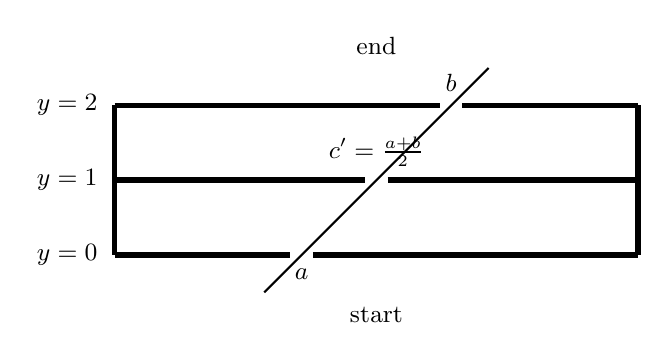
\begin{tikzpicture}[scale=0.95]
			\tikzset{wall/.style={line width=2pt}}

			% Side walls
			\draw[wall] (-0.5,0) -- (-0.5,2);
			\draw[wall] (6.5,0) -- (6.5,2);

			% Bottom wall y=0: hole at x=2 (a ∈ A)
			\draw[wall] (-0.5,0) -- (1.85,0);
			\draw[wall] (2.15,0) -- (6.5,0);

			% Middle wall y=1: hole at x=3 (c' s.t. 2c'∈C)
			\draw[wall] (-0.5,1) -- (2.85,1);
			\draw[wall] (3.15,1) -- (6.5,1);

			% Top wall y=2: hole at x=4 (b ∈ B)
			\draw[wall] (-0.5,2) -- (3.85,2);
			\draw[wall] (4.15,2) -- (6.5,2);

			% Robot: rigid stick of length 2M passing through all three holes.
			% Endpoints at (a,0)=(2,0) and (b,2)=(4,2); midpoint (3,1)=c' ✓
			\draw[thick] (1.5,-0.5) -- (4.5,2.5);

			% Hole labels
			\node[below, font=\small] at (2,-0.05) {$a$};
			\node[above, font=\small] at (3,1.05) {$c' = \frac{a+b}{2}$};
			\node[above, font=\small] at (4,2.05) {$b$};

			% Wall labels
			\node[left, font=\small] at (-0.6,0) {$y=0$};
			\node[left, font=\small] at (-0.6,1) {$y=1$};
			\node[left, font=\small] at (-0.6,2) {$y=2$};

			% Start / end labels
			\node[font=\small] at (3,-0.8) {start};
			\node[font=\small] at (3, 2.8) {end};
		\end{tikzpicture}
	\end{center}

	Therefore, this robot can only move from the line on $y=0$ to the line on $y=2$ by passing through the line on $y=1$. The robot can only pass through the holes, so it can only move from $a \in A$ to $b \in B$ by passing through $c'$ if and only if $a + b = 2c'$, which is equivalent to $a + b = c$.
\end{proof}

\section{Optimization on Numeric Operations}

If we're counting the number of numeric operations performed on 3SUM, we can actually make it better than $O(n^2)$. Here we present an algorithm that performs $O(n^{1.5}\log n)$ numeric operations at the cost of increasing the time complexity compared to Algorithm~\ref{alg:3sum} (note the difference between counting numeric operations and measuring time complexity).

\begin{enumerate}
	\item We start with a same sorted matrix $M$ where $M[i, j] = A[i] + B[j]$.
	\item Now we split $M$ into $n/g \times n/g$ blocks of size $g \times g$.
	\item Set $L$ to be $\{a-a' \mid a,a'\in A_i \text{ for some } i\} \cup \{b-b' \mid b,b'\in B_i \text{ for some } i\}$, where $A_i$ and $B_i$ are the $i$-th blocks of $A$ and $B$ respectively. The size of $L$ is at most $2\times n/g \times g^2 = 2ng$.
	      We can afford to sort $L$, as it only takes $O(ng \log (ng))$ time.
	      \begin{lemma}
		      Given the sorded list $L$, the sorted order in any block can be deduced in 0 comparisons.
	      \end{lemma}
	      \begin{proof}
		      Assume $a+b$ and $a'+b'$ are in a same block. Then $a-a' \in L$ and $b-b' \in L$. We have
		      \[
			      a+b < a'+b' & \iff a-a' < b'-b                                   \\
		      \]
		      As both $a-a'$ and $b'-b$ are in $L$, we can deduce the sorted order of $a+b$ and $a'+b'$ without any comparison.
	      \end{proof}
	\item Similar to Algorithm~\ref{alg:3sum}, we can compare $c$ with every item in the top-right corner blocks. We can use binary search now, as sorting the blocks takes no comparisons.
	      If $c$ is in the block, we are done. Otherwise, we compare $c$ with the bottom-left corner of the block matrix to determine whether to move down or left, as it can eliminate an entire row or array of blocks.
\end{enumerate}
The number of comparisons is $O(n/g \log g)$ for each $c$, and there are $n$ values of $c$, so the total number of comparisons is $O(n^2/g \log g)$.

We want to balance $O(ng \log (ng))$ and $O(n^2/g \log g)$, which gives us $g = \sqrt{n}$, and the total number of numeric operations is $O(n^{1.5} \log n)$.
